% Diagrama 3: proceso 2 (proceso2mosaico.ipynb)
% Normalización radiométrica adaptada del método RPRN (Liu et al., 2022),
% a partir de las salidas .dim (banda Sigma0) del proceso 1.
% Cifras de la última corrida (octubre de 2026).
% Compila en Overleaf con pdfLaTeX o XeLaTeX.
\documentclass[border=12pt]{standalone}
\usepackage{iftex}
\ifPDFTeX
  \usepackage[utf8]{inputenc}
  \usepackage[T1]{fontenc}
  \usepackage[scaled]{helvet}
\else
  \usepackage{fontspec}
  \setsansfont{texgyreheros}[Extension=.otf, UprightFont=*-regular,
    BoldFont=*-bold, ItalicFont=*-italic, BoldItalicFont=*-bolditalic, Scale=0.95]
\fi
\renewcommand{\familydefault}{\sfdefault}
\usepackage{amsmath}
\usepackage{tikz}
\usetikzlibrary{arrows.meta, positioning, shapes.geometric, fit, backgrounds, calc}

\definecolor{azul}{HTML}{1F5A96}
\definecolor{morado}{HTML}{6A1B9A}
\definecolor{naranja}{HTML}{E07B00}
\definecolor{gris}{HTML}{455A64}

\begin{document}
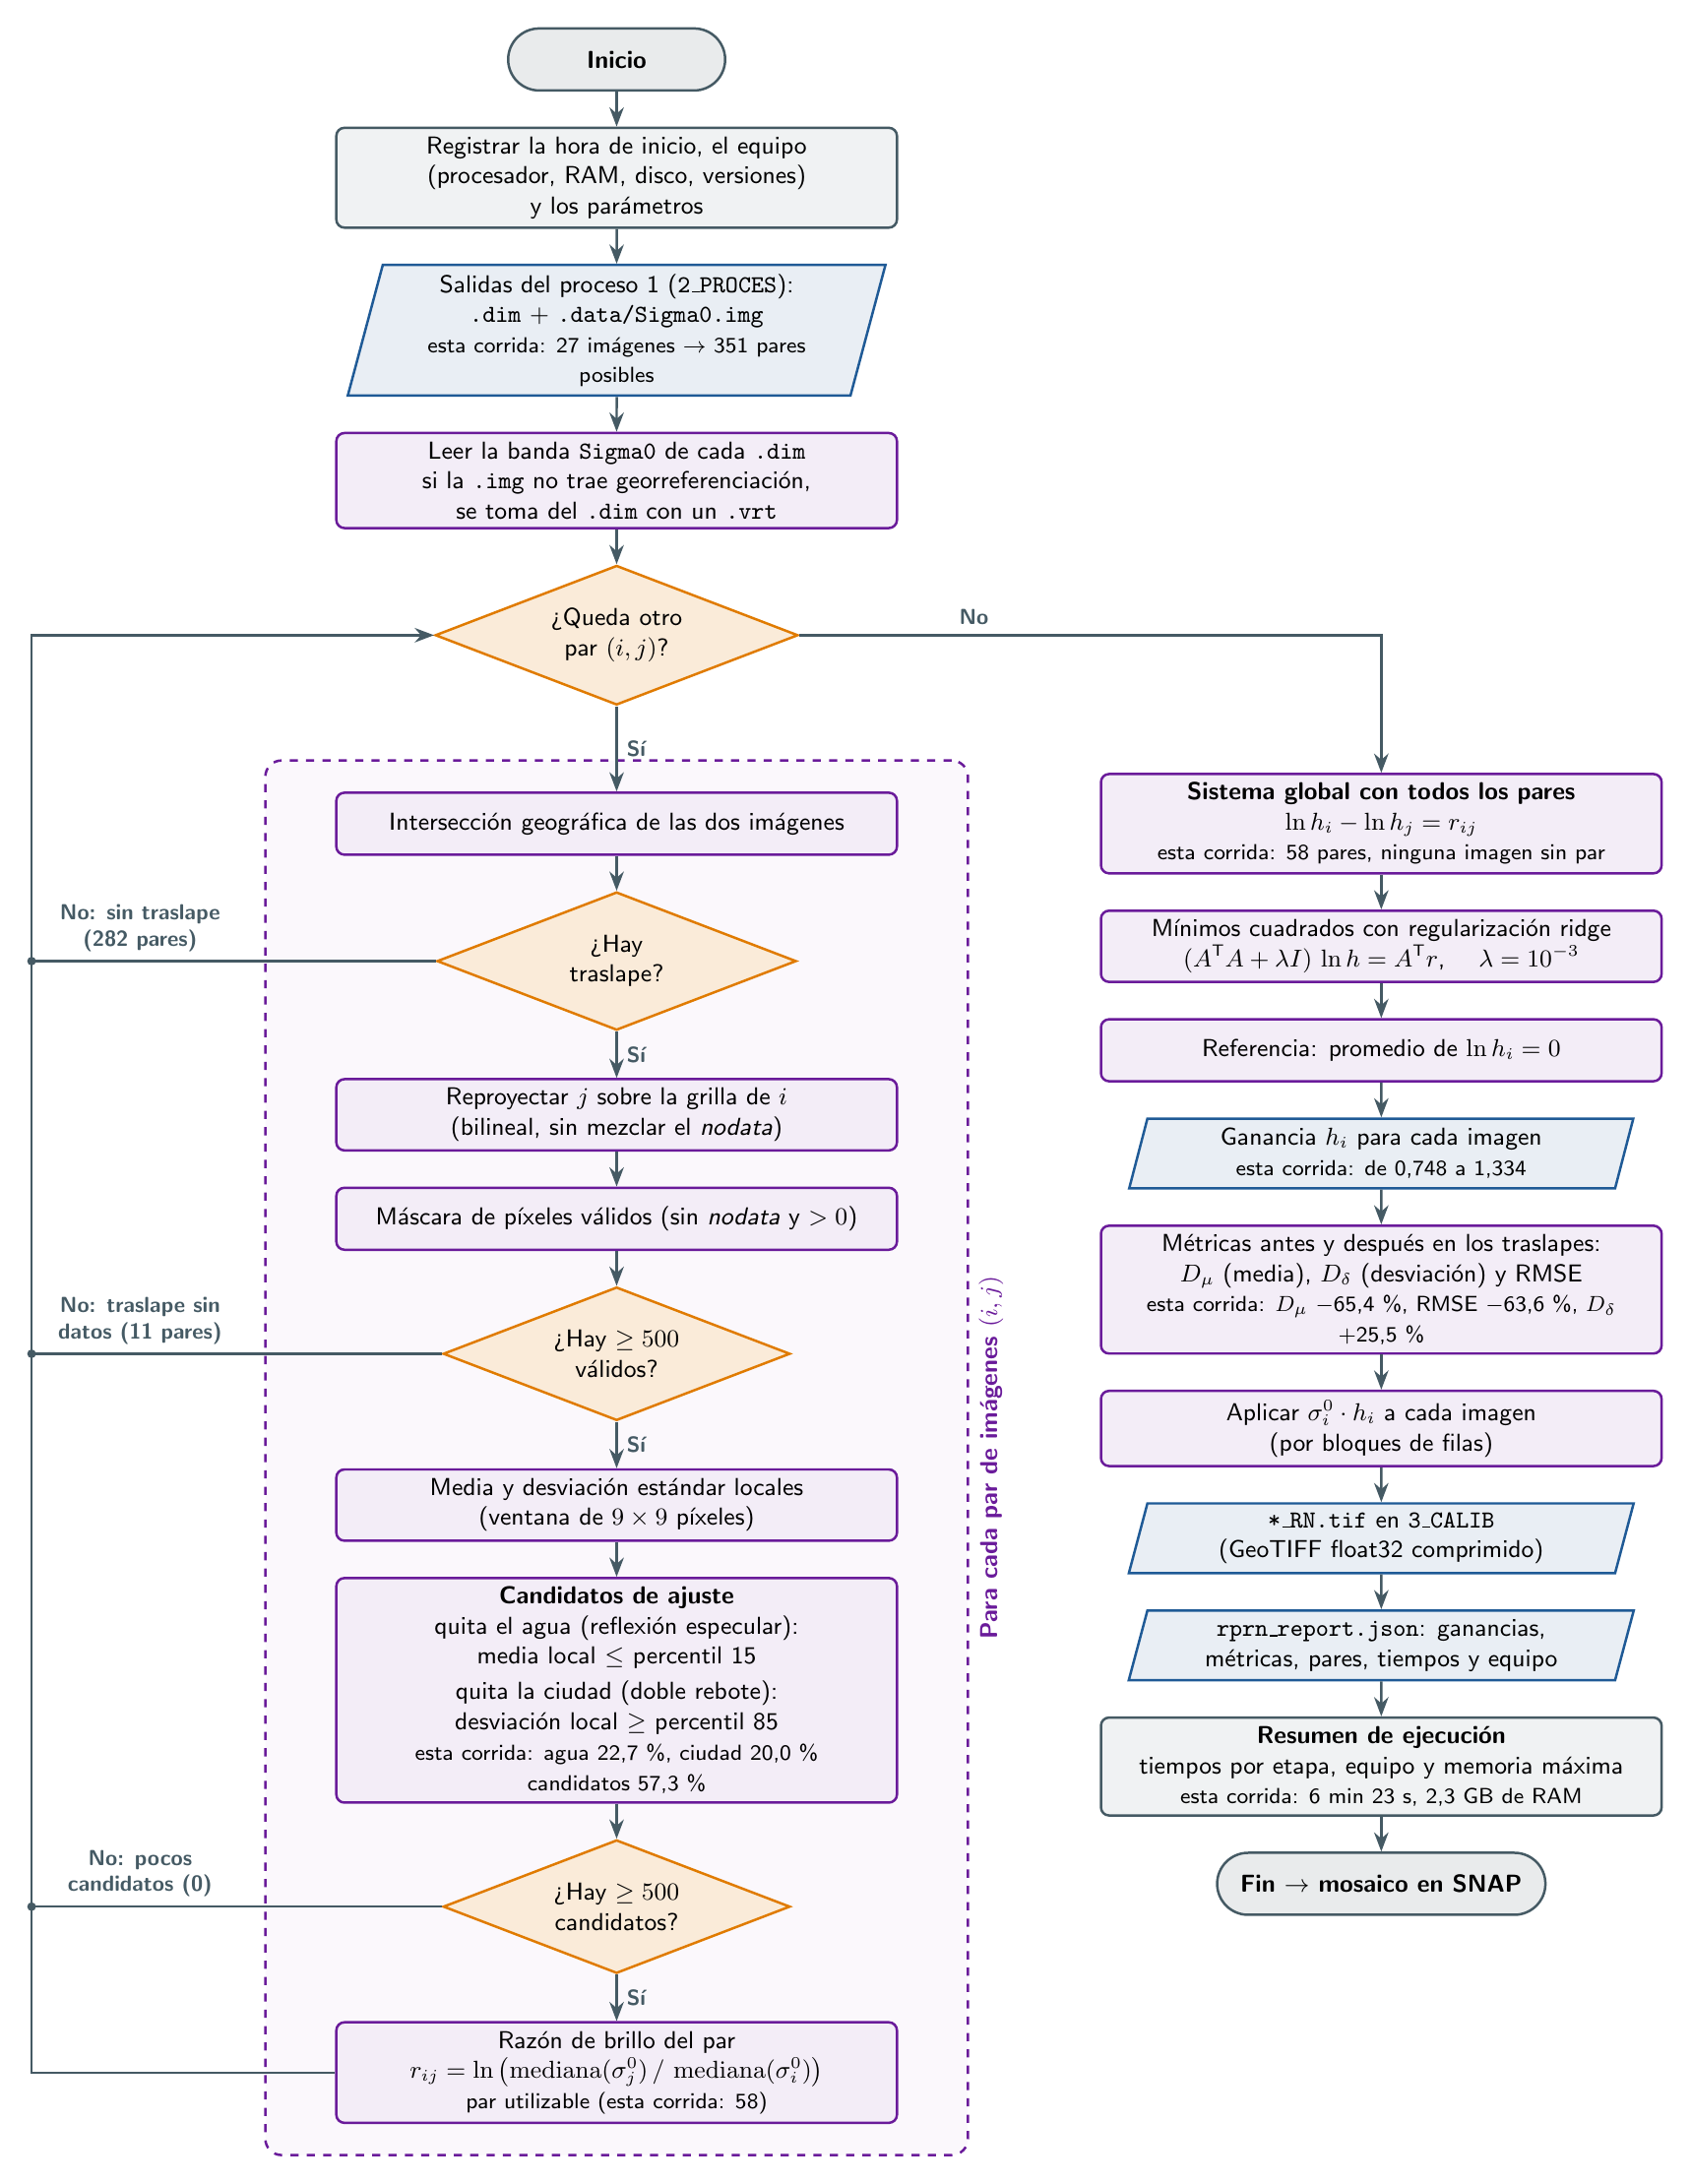
\begin{tikzpicture}[
  >=Stealth,
  node distance=4.5mm,
  proc/.style={rectangle, rounded corners=3pt, draw=morado, line width=0.9pt,
               fill=morado!8, text width=7cm, align=flush center,
               minimum height=8mm, font=\small},
  info/.style={rectangle, rounded corners=3pt, draw=gris, line width=0.9pt,
               fill=gris!8, text width=7cm, align=flush center,
               minimum height=8mm, font=\small},
  datos/.style={trapezium, trapezium left angle=75, trapezium right angle=105,
                trapezium stretches=true, draw=azul, line width=0.9pt,
                fill=azul!10, text width=5.8cm, align=flush center,
                minimum height=9mm, font=\small},
  dec/.style={diamond, aspect=2.6, draw=naranja, line width=0.9pt,
              fill=naranja!15, text width=2.9cm, align=flush center,
              inner sep=0pt, font=\small},
  term/.style={rectangle, rounded corners=4mm, draw=gris, line width=0.9pt,
               fill=gris!12, minimum width=2.8cm, minimum height=8mm,
               inner xsep=3mm, align=flush center, font=\small\bfseries},
  flecha/.style={->, line width=0.9pt, draw=gris},
  etq/.style={font=\footnotesize\bfseries, text=gris}
]

% ---------- columna 1: entradas y análisis por pares ----------
\node[term] (ini) {Inicio};
\node[info, below=of ini] (eq) {Registrar la hora de inicio, el equipo\\
  (procesador, RAM, disco, versiones)\\ y los parámetros};
\node[datos, below=of eq] (in) {Salidas del proceso 1 (\texttt{2\_PROCES}):\\
  \texttt{.dim} + \texttt{.data/Sigma0.img}\\
  \footnotesize esta corrida: 27 imágenes $\rightarrow$ 351 pares posibles};
\node[proc, below=of in] (prep) {Leer la banda \texttt{Sigma0} de cada \texttt{.dim}\\
  si la \texttt{.img} no trae georreferenciación,\\ se toma del \texttt{.dim} con un \texttt{.vrt}};
\node[dec, below=of prep] (par) {¿Queda otro\\ par $(i,j)$?};

\node[proc, below=11mm of par] (bb) {Intersección geográfica de las dos imágenes};
\node[dec, below=of bb] (tras) {¿Hay\\ traslape?};
\node[proc, below=6mm of tras] (rep) {Reproyectar $j$ sobre la grilla de $i$\\ (bilineal, sin mezclar el \textit{nodata})};
\node[proc, below=of rep] (val) {Máscara de píxeles válidos (sin \textit{nodata} y $>0$)};
\node[dec, below=of val] (nval) {¿Hay $\geq 500$\\ válidos?};
\node[proc, below=6mm of nval] (est) {Media y desviación estándar locales\\ (ventana de $9\times9$ píxeles)};
\node[proc, below=of est] (cand) {\textbf{Candidatos de ajuste}\\
  quita el agua (reflexión especular):\\ media local $\leq$ percentil 15\\[2pt]
  quita la ciudad (doble rebote):\\ desviación local $\geq$ percentil 85\\[2pt]
  \footnotesize esta corrida: agua 22,7~\%, ciudad 20,0~\%\\ \footnotesize candidatos 57,3~\%};
\node[dec, below=of cand] (n) {¿Hay $\geq 500$\\ candidatos?};
\node[proc, below=6mm of n] (ratio) {Razón de brillo del par\\
  $r_{ij} = \ln\left(\operatorname{mediana}(\sigma^0_j) \,/\, \operatorname{mediana}(\sigma^0_i)\right)$\\
  \footnotesize par utilizable (esta corrida: 58)};

\begin{scope}[on background layer]
  \node[draw=morado, dashed, line width=0.9pt, rounded corners=6pt,
        fill=morado!3, fit=(bb)(ratio), inner xsep=9mm, inner ysep=4mm] (caja) {};
\end{scope}
\node[font=\small\bfseries, text=morado, rotate=90, anchor=north]
  at (caja.east) {Para cada par de imágenes $(i,j)$};

\coordinate (L) at ($(caja.west)+(-30mm,0)$);

% ---------- columna 2: ajuste global y salidas ----------
\node[proc, right=26mm of bb] (sis) {\textbf{Sistema global con todos los pares}\\
  $\ln h_i - \ln h_j = r_{ij}$\\
  \footnotesize esta corrida: 58 pares, ninguna imagen sin par};
\node[proc, below=of sis] (ridge) {Mínimos cuadrados con regularización ridge\\
  $(A^{\mathsf T}A + \lambda I)\,\ln h = A^{\mathsf T} r$, \quad $\lambda = 10^{-3}$};
\node[proc, below=of ridge] (ancla) {Referencia: promedio de $\ln h_i = 0$};
\node[datos, below=of ancla] (h) {Ganancia $h_i$ para cada imagen\\
  \footnotesize esta corrida: de 0,748 a 1,334};
\node[proc, below=of h] (met) {Métricas antes y después en los traslapes:\\
  $D_\mu$ (media), $D_\delta$ (desviación) y RMSE\\
  \footnotesize esta corrida: $D_\mu$ $-$65,4~\%, RMSE $-$63,6~\%, $D_\delta$ +25,5~\%};
\node[proc, below=of met] (apl) {Aplicar $\sigma^0_i \cdot h_i$ a cada imagen\\ (por bloques de filas)};
\node[datos, below=of apl] (out) {\texttt{*\_RN.tif} en \texttt{3\_CALIB}\\ (GeoTIFF float32 comprimido)};
\node[datos, below=of out] (rep2) {\texttt{rprn\_report.json}: ganancias,\\ métricas, pares, tiempos y equipo};
\node[info, below=of rep2] (res) {\textbf{Resumen de ejecución}\\
  tiempos por etapa, equipo y memoria máxima\\
  \footnotesize esta corrida: 6 min 23 s, 2,3 GB de RAM};
\node[term, below=of res] (fin) {Fin $\rightarrow$ mosaico en SNAP};

% ---------- flechas ----------
\draw[flecha] (ini) -- (eq);
\draw[flecha] (eq) -- (in);
\draw[flecha] (in) -- (prep);
\draw[flecha] (prep) -- (par);
\draw[flecha] (par) -- node[etq, right]{Sí} (bb);
\draw[flecha] (bb) -- (tras);
\draw[flecha] (tras) -- node[etq, right]{Sí} (rep);
\draw[flecha] (rep) -- (val);
\draw[flecha] (val) -- (nval);
\draw[flecha] (nval) -- node[etq, right]{Sí} (est);
\draw[flecha] (est) -- (cand);
\draw[flecha] (cand) -- (n);
\draw[flecha] (n) -- node[etq, right]{Sí} (ratio);

% retornos al siguiente par (cada "No" se anota en el reporte)
\draw[flecha] (ratio.west) -| (L |- par.west) -- (par.west);
\draw[line width=0.9pt, draw=gris] (tras.west) -- (L |- tras.west);
\node[etq, above, align=center] at ($(L |- tras.west)+(14mm,0)$) {No: sin traslape\\ (282 pares)};
\fill[gris] (L |- tras.west) circle (1.6pt);
\draw[line width=0.9pt, draw=gris] (nval.west) -- (L |- nval.west);
\node[etq, above, align=center] at ($(L |- nval.west)+(14mm,0)$) {No: traslape sin\\ datos (11 pares)};
\fill[gris] (L |- nval.west) circle (1.6pt);
\draw[line width=0.9pt, draw=gris] (n.west) -- (L |- n.west);
\node[etq, above, align=center] at ($(L |- n.west)+(14mm,0)$) {No: pocos\\ candidatos (0)};
\fill[gris] (L |- n.west) circle (1.6pt);

% paso al ajuste global
\draw[flecha] (par.east) -- node[etq, above, pos=0.3]{No} (par.east -| sis.north) -- (sis.north);
\foreach \a/\b in {sis/ridge, ridge/ancla, ancla/h, h/met, met/apl, apl/out, out/rep2, rep2/res, res/fin}
  \draw[flecha] (\a) -- (\b);

\end{tikzpicture}
\end{document}
